\documentclass{article}

\usepackage{graphicx}
\usepackage{caption}
\usepackage{rotating}
\usepackage{float}
\usepackage[margin=0.8in]{geometry}
\usepackage[section]{placeins}
\usepackage[hidelinks]{hyperref}
\usepackage{sectsty}
\sectionfont{\clearpage}
\usepackage{csquotes}
\MakeOuterQuote{"}

\setlength{\parskip}{0.3em}
\usepackage{xcolor}
\usepackage{listings}
\lstset{
	language=Verilog,
	frame=single,
	basicstyle=\small,
	keywordstyle=\color{blue}\small,
	stringstyle=\color{Maroon}\small,
	commentstyle=\color{OliveGreen}\small,
	breaklines=true,
	postbreak=\raisebox{0ex}[0ex][0ex]{\ensuremath{\color{red}\hookrightarrow\space}}
}

\title{FPGABoy Documentation}
\author{Luke Wren}

\begin{document}

\pagenumbering{gobble}
\maketitle
\tableofcontents
\newpage
\pagenumbering{arabic}

\section{Introduction}

FPGABoy is an open source portable games console, designed from scratch. It is also...
\begin{itemize}
\item An open source PCB layout
\item Designed with KiCAD open source PCB software
\item An open source CPU, graphics and bus architecture
\item Based on the RISC-V open source instruction set
\item Synthesised, placed and routed with iCEStorm open source FPGA toolchain
\item It's open source
\end{itemize}

\begin{displayquote}
\textit{If you say open source one more time I'm gonna nut instantly} - Oscar Wilde
\end{displayquote}

\subsection{Digital Design}

\begin{figure}[!htb]
\caption{System-level architecture}
\label{diagram:system_arch}
\centering
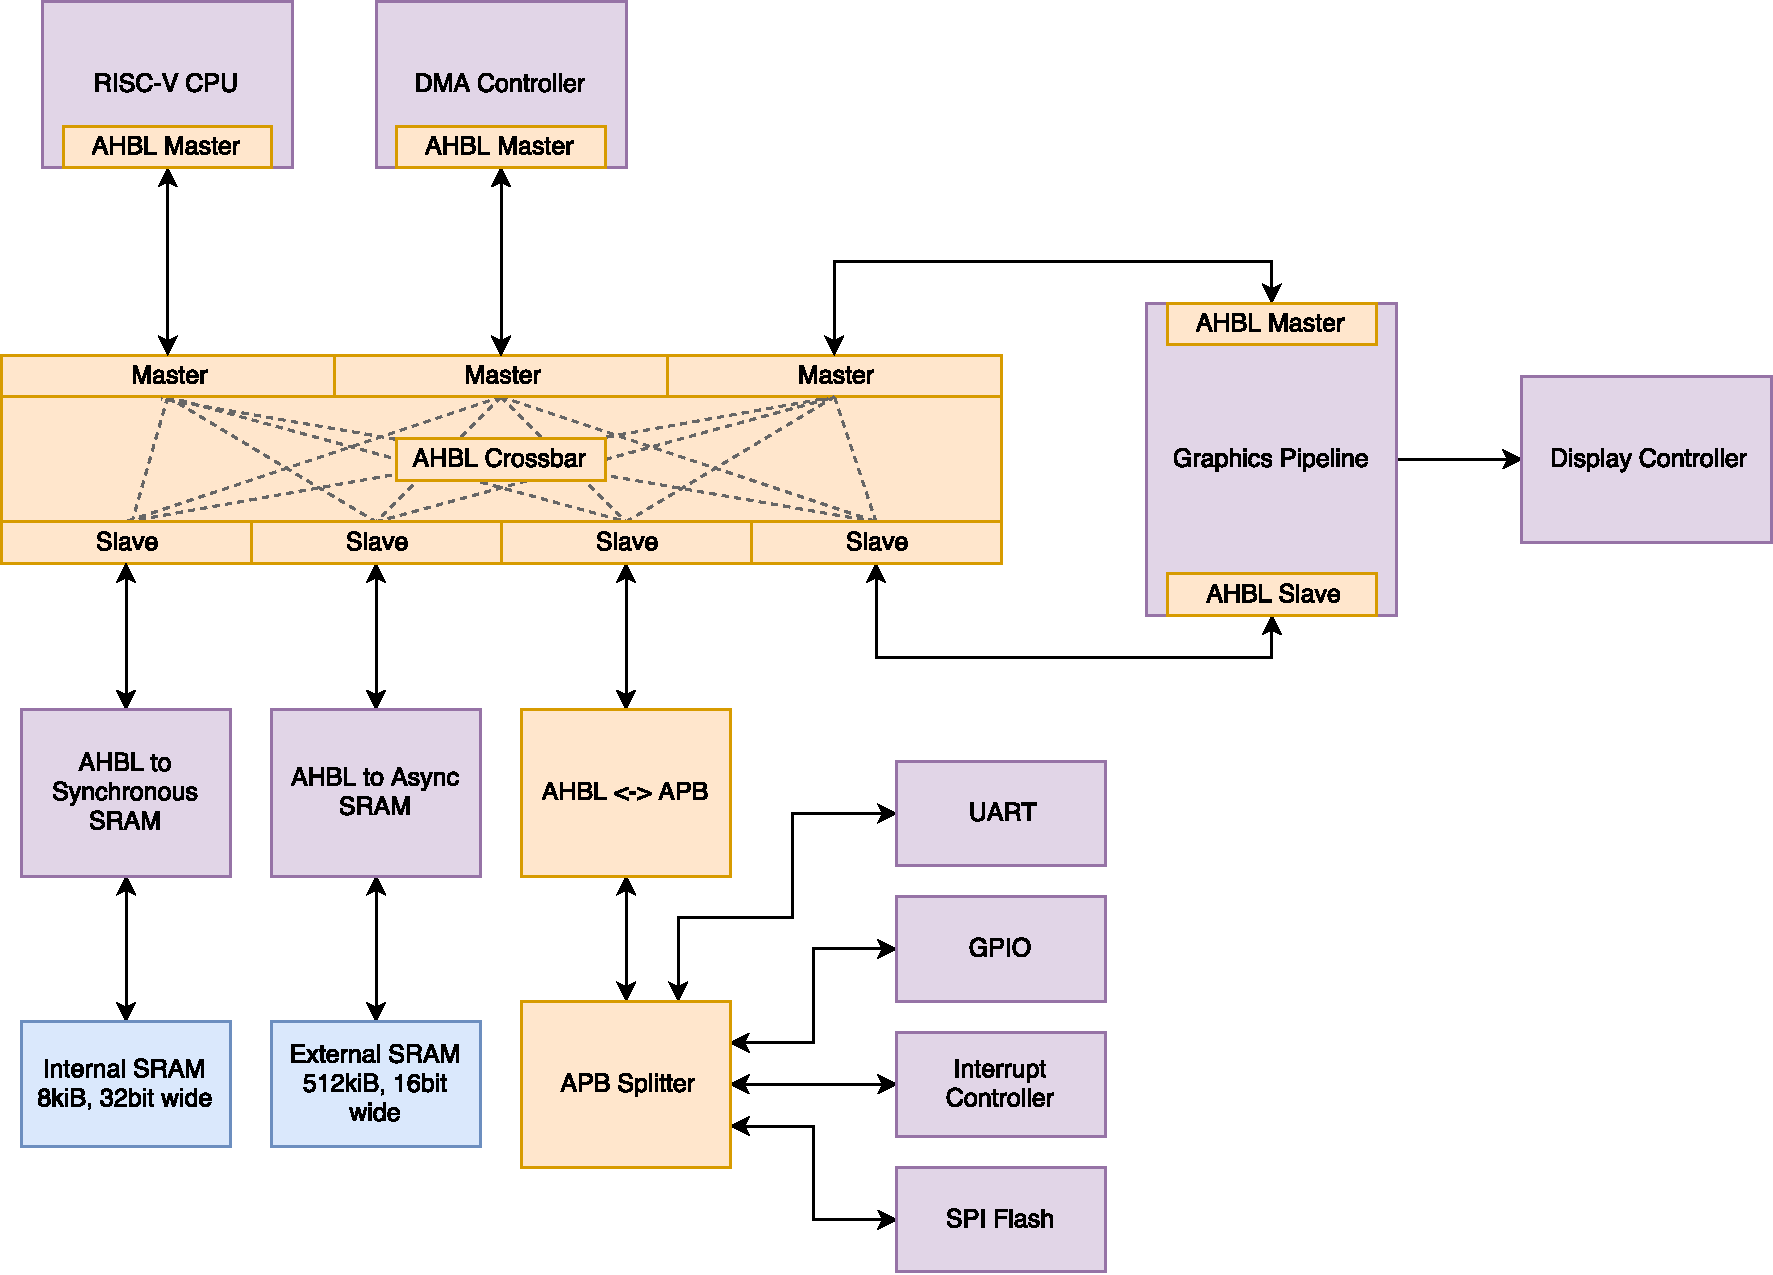
\includegraphics[width=0.7\textwidth]{diagrams/system_arch.pdf}
\end{figure}

The heart of the design is a Lattice iCE40-HX8k FPGA, containing 7680 LUT4s and flipflops. The logic was designed in synthesisable Verilog, with no dependencies on FPGA vendor IP; the contents of this GitHub repository could be taped out onto a chip. This includes:

\begin{itemize}
\item RV32IC-compatible 32-bit CPU design
	\begin{itemize}
	\item RISC-V instruction set
	\item 32I: base integer ISA profile
	\item C: compressed instruction extension, for higher code density
	\item Vectored interrupts (save/restore of PC, RA only)
	\item 5-stage pipeline, similar to textbook RISC
	\item Single AHB-lite master port
	\end{itemize}
\item Graphics pipeline
	\begin{itemize}
	\item Don't expect much, it's about as powerful as a Gameboy Advance
	\item Includes some MODE7-like functionality which allows drawing perspective-mapped textured planes, by providing per-scanline affine texture transformation. Think MarioKart
	\end{itemize}
\item AMBA 3 AHB-lite compatible multi-master busfabric
\item Peripherals:
	\begin{itemize}
	\item DMA master
	\item External asynchronous SRAM controller (GS74116 or similar)
	\item Display controller (ILI9341)
	\item SPI flash controller with direct memory-mapped access
	\item GPIO (bitbanging, peripheral muxing)
	\item Interrupt controller
	\item UART
	\item PWM
	\item Basic audio: voices + samples, noise-shaped PWM output
	\end{itemize}
\end{itemize}

Some attempt is made in this document to describe the operation of these blocks, but if you are looking for nitty-gritty detail, the best documentation is the files ending with \texttt{.v}.

That a free synthesis tool can cram all this logic into one of the cheapest FPGAs on the market is tremendously impressive. Hopefully we will one day have a situation similar to software compilers, where free tools such as GCC are industry standards.

\subsection{PCB}

The board is a 4-layer stackup:

\begin{enumerate}
\item Signal + GND Fill
\item GND plane
\item Power planes
\item Signal + GND Fill
\end{enumerate}

It is intended to be suitable for low-cost PCB prototyping services such as iTead. Board dimensions are 50mm $\times$ 50mm, which fits into the cheapest size category on iTead. For the most part, it sticks to the following minimum specifications:

\begin{itemize}
\item Track width 0.15mm
\item Copper-copper clearance 0.15mm
\item Soldermask-copper clearance 0.1mm
\item Soldermask width 0.1mm
\item Via drill 0.3mm
\item Annular ring 0.15mm (i.e. via diameter 0.6mm)
\end{itemize}

The only exception is some 0.5mm vias underneath the BGA. Strictly this is out of specification for iTead, but they claim to have a 90 $\mu$m drill registration, so we'll see how it goes.

The iCE40-HX8k FPGA is packaged in a 256-pin 0.8mm BGA, which \textit{can be} reflowed by a hobbyist with a hot air gun or a frying pan (best to choose a HASL finish so that contacts are pretinned). The 132-pin 0.5mm BGA has sufficient IO for our needs, but iTead does not manufacture at the tolerance required for such a fine pitch.


\subsection{Licensing}

The Verilog source to this project has no dependencies, and is distributed under the DWTFPL version 3. This is a \textit{very} permissive open-source licence, and its text is included in full at the top of the source files. This license is very similar to the original DWTFPL, which more readers may be familiar with, but has an added indemnification clause.

This license is also known by its more formal name, as the "Do What The Fuck You Want To And Don't Blame Us Public License".

\section{CPU Architecture}

Hazard5 is a 32-bit processor based on the RISC-V instruction set architecture. It accesses the system through a single AMBA 3 AHB-lite master port. Those familiar with the textbook 5-stage RISC pipeline will find Hazard5 mostly straightforward, but hopefully will still find some interesting tricks. We will use the following symbols to refer to the 5 stages:

\begin{itemize}
\item \texttt{F}: fetch
\item \texttt{D}: decode
\item \texttt{X}: execute
\item \texttt{M}: memory access (load/store)
\item \texttt{W}: register writeback, fetch address generation
\end{itemize}


Hazard5 supports the RV32IC instruction set, which is variable-width. The narrower instructions help the core to maintain instruction throughput whilst sharing bus access between fetch and load/store; RV-C reduces fetch bandwidth by around 25\%.

Branches are speculated, but there is no dynamic branch predictor. Instead, we use static prediction scheme described in the RV ISA manual:

\begin{itemize}
\item Backward branches predicted taken; hopefully, loops run at least twice on average.
\item Forward branches predicted not taken; the ISA manual advises compilers should put more-likely code on this path.
\end{itemize}


% \newpage

% \begin{center}
% 	\begin{sideways}
% 		\begin{minipage}{\textheight}
% 			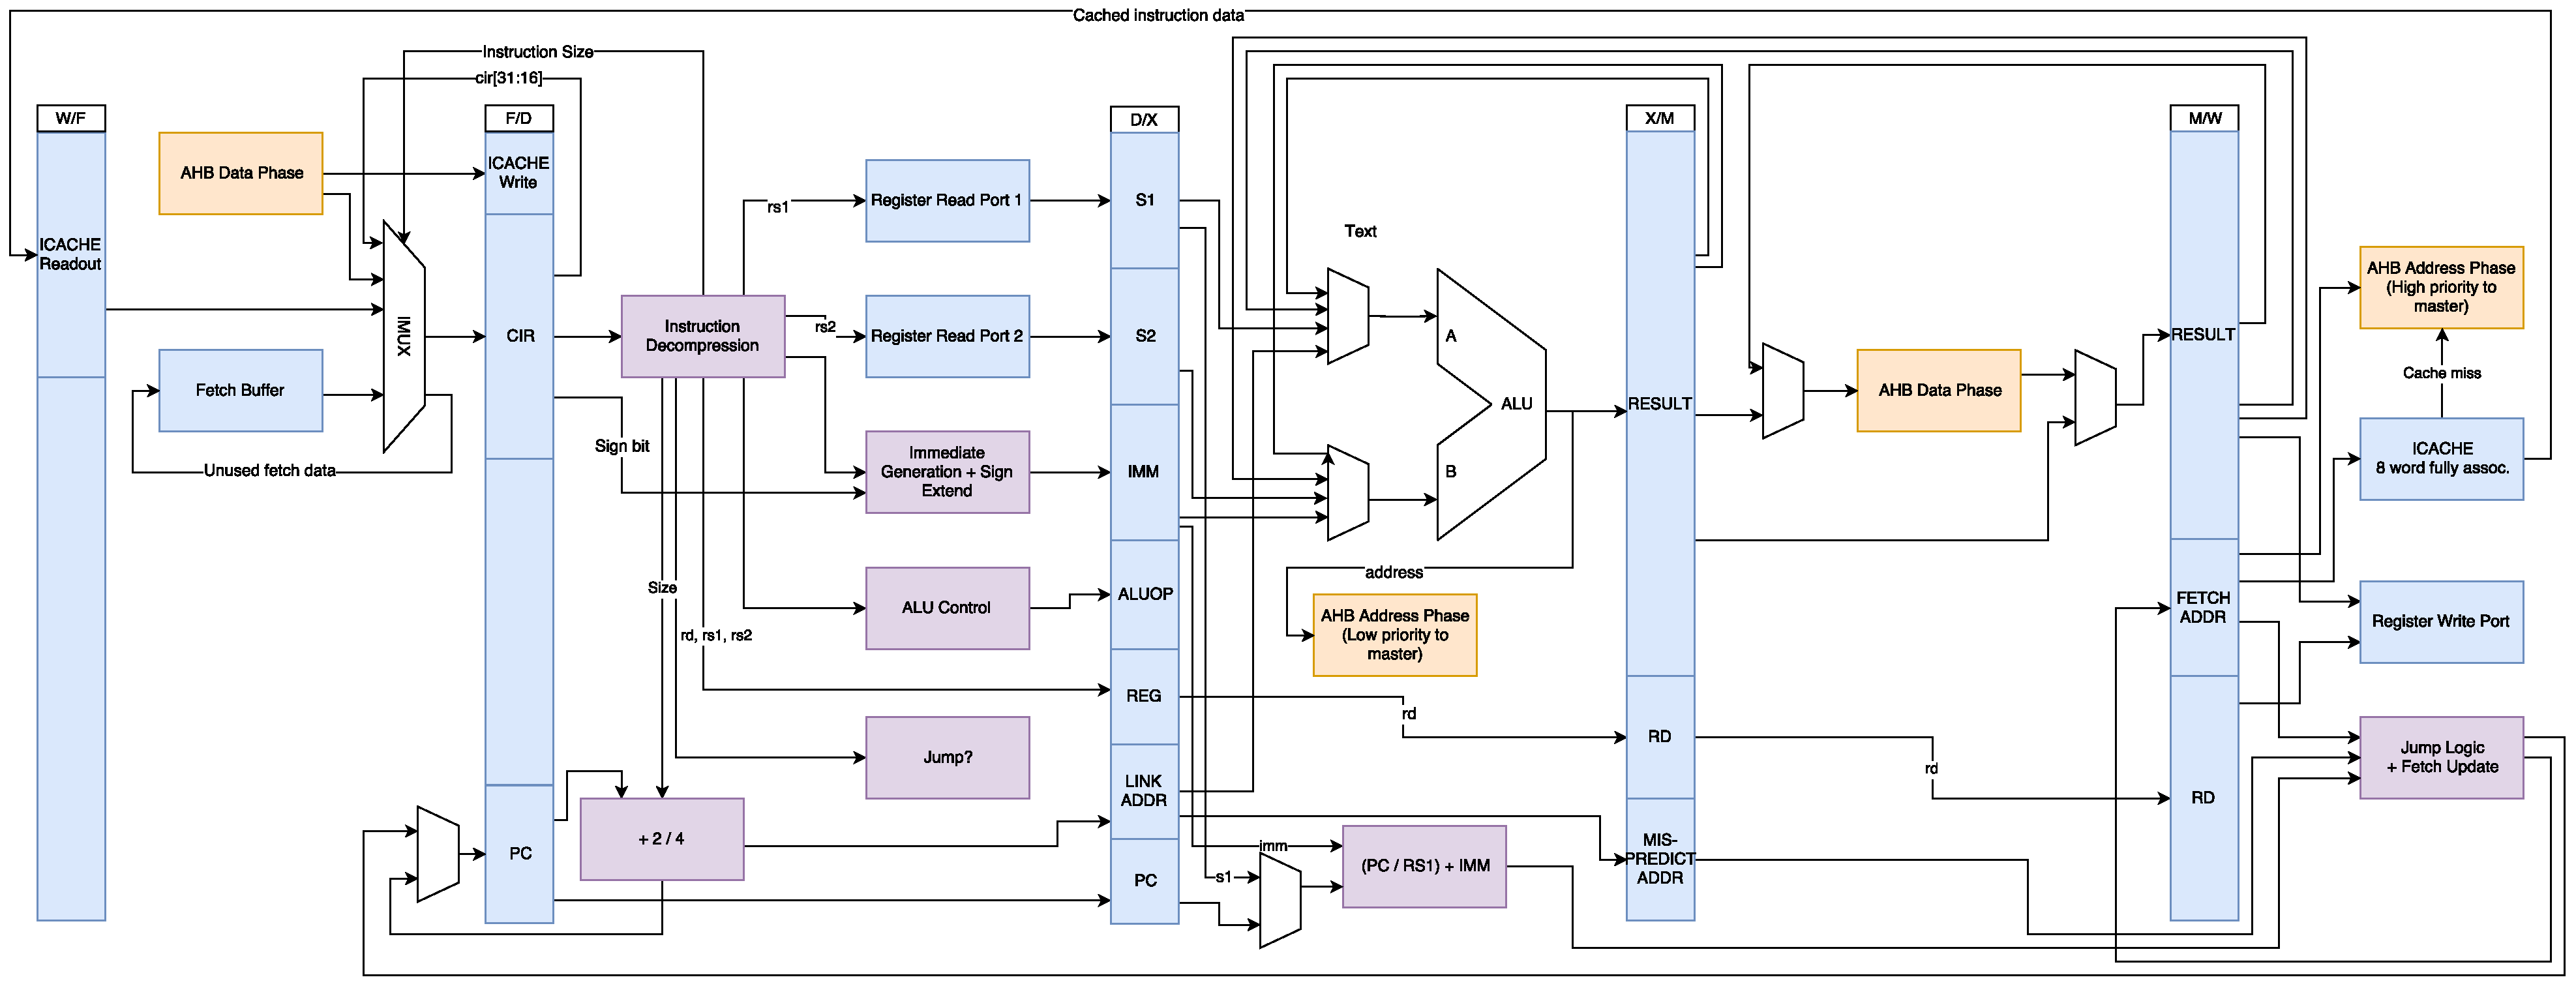
\includegraphics[width=\textheight]{diagrams/cpu_full.pdf}
% 			\captionof{figure}{Hazard5 architectural block diagram}
% 			\label{diagram:cpu_pipeline}
% 		\end{minipage}
% 	\end{sideways}
% \end{center}

% \newpage


TODO: frontend and backend diagrams
\subsection{Frontend}
\label{section:frontend}

The front end consists of stage \texttt{F} and an additional stage which performs the AHB address phase, and can be considered part of \texttt{W}. Its purpose is to feed \texttt{D} with instructions, whilst meeting the following constraints:

\begin{itemize}
	\item No combinational path from AHB-lite data-phase to address-phase (e.g. \texttt{hready} $\to$ \texttt{htrans})
	\item AHB-lite compliant: no unaligned transfers, no deassertion or change of active requests
	\item Provide up to 32 bits of instruction data per clock in steady state, even if instructions are unaligned
	\item 0-cycle jump/flush to AHB address phase assertion (with minimal logic on this path)
	\item No performance penalty for unaligned jump to 16-bit instruction
	\item Attempt to maintain performance when competing with the load/store unit and AHB-lite busmaster peers
\end{itemize}

A RISC-V *C instruction stream is not naturally-aligned, by which we mean instruction address modulo instruction size is not always zero. This complicates the front end considerably, and we spend gates here to optimise the common case of sequential execution, and to lessen the effects of fetch starvation due to load-store activity.

To meet these constraints, the frontend performs almost exclusively word accesses, which must be aligned. The only exception is a jump (or similar, e.g. mispredict recovery) to a non-word-aligned address. In this case, a halfword fetch from the target address is performed.

\subsubsection{Prefetch Queue}

The frontend queues up fresh instruction data which is waiting to be decoded. The pipelined nature of AHB-lite means that the bus transfers run ahead of \texttt{D} by at least two clocks, and the prefetch queue is able to buffer these in-flight transfers if \texttt{D} stalls against a later pipe stage. The queue also decouples \texttt{D}'s stall logic (which is a function of \texttt{hready}) from the address phase request, and finally, the queue helps keep \texttt{D} supplied with instructions while the busmaster is busy with load/stores from \texttt{X}.

There are three parts to the queue:

\begin{itemize}
	\item A 32-bit FIFO. The depth is configurable, and can be as little as 1 word.
	\item A halfword buffer which may store the higher-addressed half of a recently-popped FIFO word
	\item The upper half of the current instruction register (\texttt{CIR}), if the previous instruction was 16-bit
\end{itemize}

These three sources should service the majority of instruction fetches, and fresh bus data is written only to the FIFO. However, in the case of jumps, flushes, and other fetch starvation, bus data can be forwarded directly to \texttt{CIR}.

\subsubsection{Program Counter}

Hazard5 does \textit{not} use the program counter (\texttt{PC}) for code fetching, during sequential execution. \texttt{PC} is used exclusively for the link value in \texttt{JAL(R)}, mispredict recovery, and PC-relative addressing; it is physically located in \texttt{D}.

The frontend fetches instruction data from consecutive word-aligned addresses, paced by backpressure from the instruction FIFO; \texttt{PC} is not involved. However, as a special case, it \textit{does} need the full jump target address (which becomes the new \texttt{PC}), as unaligned jumps require special attention.

\subsubsection{Arbitration of Fetch and Load/Store}
\label{section:fetch_ls_arb}

The single AHB master port asserts transactions from two sources: the frontend, whose address phase is in \texttt{W}, and the load/store unit, whose address phase is in \texttt{X}. Frontend requests may be linear or non-linear (e.g jumps). The rules are:

\begin{enumerate}
	\item If a jump or mispredict recovery is asserted by \texttt{M}, this wins.
	\begin{itemize}
		\item Any requests from earlier stages are logically later in program order.
		\item If \texttt{M} wants to jump then these instructions are being executed in error, so should certainly not be permitted to access the bus.
	\end{itemize}
	\item Else if a load/store is asserted by \texttt{X}, this wins.
	\begin{itemize}
		\item Stalling instruction fetch \textit{may} be covered by the prefetch queue, in which case we've lost nothing
		\item Stalling a load/store will always increase execution time
		\item If instead \texttt{X} stalled, and instruction fetch ran ahead, what would we do with the fetched instructions?
	\end{itemize}
	\item Otherwise, perform any other access requested by the frontend.
	\begin{itemize}
		\item Always Be Fetching
	\end{itemize}
\end{enumerate}

\subsubsection{Jumps and Branches}

Due to the pipelined nature of AHB, we are unable to jump or to take branches in fewer than 2 cycles (without some fairly sophisticated prediction):

\begin{itemize}
\item Cycle 0: AHB address phase to fetch jump/branch instruction
\item Cycle 1: AHB data phase for fetch of jump/branch. Next instruction is in address phase concurrently.
\item Cycle 2: Jump/branch instruction is now available to \texttt{D}
	\begin{itemize}
		\item (Quickly) use to control the new address phase
		\item The immediately following instruction is already in data phase
	\end{itemize}
\item Cycle 3: data phase for jump target instruction
\end{itemize}


We've paid one penalty cycle in the pipeline (cycle 2), and also made one wasted code fetch.

Jumps are physically taken in \texttt{W}, directly in front of the fetch address generator. There are two reasons to jump:

\begin{itemize}
	\item Inspecting the \texttt{CIR} in \texttt{F/D} pipe register (\texttt{JAL}, speculated taken branches)
	\item Inspecting \texttt{X/M} pipe register (\texttt{JALR}, branch mispredict)
\end{itemize}

\texttt{JALR} (indirect jump) is taken later because it uses the register file and the ALU to compute its target.

If both of these sources attempt to jump in the same cycle, \texttt{X/M} takes priority, since it is executing an older instruction. In both cases, the part of the pipeline in the hazard shadow is invalidated; i.e., \texttt{W} $\to$ \texttt{F}, or \texttt{W} $\to$ \texttt{X}. Invalidation is performed by clobbering the pipeline control signals in such a way that these instructions will have no side effects.

The branch prediction scheme is static: take backward branches, and do not take forward branches. The cycle costs are as follows:

\begin{center}
\begin{tabular}{l c}
\hline
Jump Type & Cycles (Execution + Penalty) \\
\hline
Direct jump & 2 \\
Predicted, non-taken branch & 1 \\
Predicted, taken branch (same as jump) & 2 \\
Indirect jump & 4 \\
Branch mispredict & 4 \\
\hline
\end{tabular}
\end{center}

Upon jumping, we need some mechanism to invalidate parts of the pipeline: this is described in section \ref{section:stalling_flushing}.

\subsubsection{Instruction Barrier (FENCE.I)}

If the program stores to instruction addresses which will be imminently executed, and therefore exist in the prefetch queue, the stale instruction will be executed.. This cannot be solved by decoding FENCE.I as a nop, and requires special handling.

Hazard5 decodes FENCE.I as "jump to \texttt{PC} + 4". The jump invalidates the prefetch queue, and the following instruction will be re-fetched from memory.

\subsection{Operand Bypass}

Hazard5 provides a multiplexed operand bypass (forwarding) network. Register writes by a given instruction must always be visible to later instructions, even \textit{before} the first instruction reaches the register writeback stage. This is shown as multiplexers on the ALU inputs in figure \ref{diagram:cpu_pipeline}.

This removes, or at least shortens, read-after-write data hazards in the pipeline, and allows us to approach one clock-per-instruction execution rates. Without bypassing, only one instruction could be present in $\left\{ \texttt{D}, \texttt{X}, \texttt{M}, \texttt{W} \right\}$ at a time, giving a CPI of 4.

The following bypasses are available: (notation: pipe register $\to$ pipestage logic)

\begin{itemize}
	\item \texttt{X/M} $\to$ \texttt{X}
	\item \texttt{M/W} $\to$ \texttt{X}
	\item \texttt{M/W} $\to$ \texttt{M}
	\item \texttt{M/W} $\to$ \texttt{D} (internal bypass in register file for write port $\to$ read port)
\end{itemize}

To control the bypassing, some of the register specifiers from \texttt{CIR} are passed down the pipeline alongside the data. \texttt{rs1, rs2, rd} (operand sources and destination) are passed down as far as \texttt{X}. \texttt{rs2, rd} make it to \texttt{M}, and \texttt{rd} makes it to \texttt{W}.

These serve the following purposes:

\begin{itemize}
	\item \texttt{rd} is needed in \texttt{W} anyway, for performing the actual writeback
	\item \texttt{X} looks at the two operand source registers it depends on, and then glances across at the \texttt{rd}s awaiting writes in \texttt{M} (i.e. its own output) and \texttt{W} (i.e. a load output, or an \texttt{X} output one cycle prior).
	\item \texttt{M} Looks at the \texttt{src} register for a store (encoded in the \texttt{rd2} specifier field), and will look at the pending register write in \texttt{W}, which will be either a load result or a prior \texttt{X} result.
\end{itemize}

Architecturally, it may be preferable to perform these bypasses earlier, since RISC-V makes operand decode very simple, with fixed bitfield position for rd1, rd2. That is, put the muxes between the register file and the \texttt{D/X} pipe register, and move the taps to make the hazards work. However, we want the register file to support BRAM inference on iCE40 FPGAs, as we otherwise use about 15\% of the flops on the device just to implement the registers. iCE40s have a synchronous BRAM read port, so the muxes end up after the "pipe register", i.e. the BRAM output registers.

The upshot is:

\begin{itemize}
	\item Back-to-back ALU operations execute at 1 CPI
	\item Loads execute at 2 CPI if they are immediately required by the ALU. 1 CPI otherwise.
	\item Stores execute at 1 CPI
	\item In a load-store pair, the load takes only one cycle, since the \texttt{M} stage has cyclic forwarding
\end{itemize}

\subsection{Pipeline Stalling and Flushing}
\label{section:stalling_flushing}

Our terminology: stalling means a pipeline stage does not advance its state until some blocking condition has cleared. The instruction residing in this stage will not progress to the next stage, and the previous stage will not write \textit{its} instruction into this stage. Flushing is when in-flight instructions in some stages are replaced with NOPs, and their results are discarded.

The frontend is decoupled from other stages' stall logic via the prefetch queue. This is important: \texttt{hready} is an input to that stall logic, and the the frontend's address-phase request must not be a function of \texttt{hready}.

The frontend may not be able to immediately accept a jump request, which may cause other pipe stages to stall if it is low. One cause is the frontend holding an existing address-phase request stable until the cycle \textit{after} \texttt{hready}, which is required for AHB-lite compliance.

For the backend, the stall logic is more intricate, as signals such as \texttt{hready} are used in-cycle to determine whether an instruction progresses to the next pipeline stage:

\begin{itemize}
	\item \texttt{D}:
	\begin{itemize}
		\item \texttt{CIR} does not contain a valid instruction (either no data, or half of a 32-bit instruction)
		\item \texttt{D} asserts jump, but frontend rejects the jump request
		\item \texttt{X} is stalled
	\end{itemize}
	\item \texttt{X}:
	\begin{itemize}
		\item \texttt{hready} low and \texttt{X} address-phase request asserted
		\item RAW hazard on \texttt{M}
		\item \texttt{M} is stalled
	\end{itemize}
	\item \texttt{M}:
	\begin{itemize}
		\item \texttt{hready} low and data-phase active
		\item \texttt{M} asserts jump, but frontend rejects the jump request
	\end{itemize}
	\item \texttt{W}: does not stall
\end{itemize}

If a given stage is stalled, but the following stage is not, it must insert a bubble. Bubbles are created by zeroing out control fields, such as \texttt{rd}, so that the following stage will have no side effects on the next cycle.

There are two cases where we must flush:

\begin{itemize}
	\item Branch/jump taken from \texttt{D}; frontend invalidates prefetched data
	\item Jump/mispredict taken from \texttt{M}; must flush frontend, \texttt{D}, \texttt{X}
\end{itemize}

And the flushing mechanisms for each stage are as follows:
\begin{itemize}
	\item \texttt{D}: destination register \texttt{rd} cleared, which makes result invisible to register file and operand bypass. \texttt{memop}, \texttt{branchcond} pipe flags are cleared.
	\item \texttt{X}: same as \texttt{D} (except for \texttt{branchcond}, which does not pass on to \texttt{M} anyway.
\end{itemize}

Flushing and bubble insertion are very similar; flushing is like multiple stages inserting bubbles into each other, clobbering any contained instructions.

\subsection{Unaligned Memory Accesses}

Alignment is the constraint that the address of a memory access be equal to zero, modulo some size. Where no size is specified, we refer to \textit{natural} alignment, i.e. modulo the size of this particular memory operation. RISC-V requires that memory is byte-addressable.

The frontend goes to some length (section \ref{section:frontend}) to maintain high throughput. RV-C instruction streams are \textit{always} unaligned, and \textit{every} instruction must be fetched before it is executed, so Amdahl says it's worth it.

As load/stores are less than 100\% of all instructions, and generally much less than 100\% of these are unaligned, Hazard5 does not have hardware support for unaligned load/stores. These are trapped (TODO) and handled in software if and when they occur.

\subsection{Interrupts and Exceptions}

This section is very much still TBD. (TODO)

Hazard5 will have non-nested priority vectored interrupts, with no register saving, apart from \texttt{ra} (\texttt{x2}; link/return address register) and the \texttt{PC}. Interrupts and exceptions will be implemented with the early jump hardware, so behave as a \texttt{D}-sourced jump.

Interrupts/exceptions are implemented as a jump into the vector table. The table is a block of aligned 32-bit instructions, which will most likely be JAL, meaning ISRs must be within $\pm$1 MiB of the vector table. As well as jumping into the table, the interrupt hardware stashes the \texttt{PC} and \texttt{ra} into shadow registers; the second requires a register file read, and the pipeline slot of the (victim) instruction in \texttt{D} is used to perform this read. \texttt{PC} is immediately clobbered by the jump into the table, and \texttt{ra} is clobbered with the magic value 0xffffffff, which is otherwise an invalid return address as its LSB is set.

Upon encountering a \texttt{jalr} to 0xffffffff (most likely a \texttt{ret}), the saved \texttt{PC} and \texttt{ra} are saved.

Consequently, ISRs may not generate exceptions, such as unaligned accesses. TODO: should have some kind of non-returning hardfault exception to deal with things like this.

\subsection{Possible Performance Gains}

This section lists ideas of potential improvements which are waiting for synthesis + timing reports before I make a decision, or waiting for a decent regression test suite and working processor before I make complex changes.

\begin{itemize}
	\item If a jump/exception is asserted by \texttt{D}, or a jump/branch/mispredict recovery by \texttt{M}, code fetch wins over a load/store.
	\begin{itemize}
		\item The jump will always insert a fetch bubble due to the pipelined nature of AHB-lite
		\item A stalled load/store in \texttt{X} will then execute in this bubble
		\item This saves a cycle
		\item However, as jumps may write a link address back to the register file, and \texttt{X} is stalled, the jump must remain in \texttt{D} so that it eventually progresses down the pipeline. However, its "jump" side effect needs to be disabled once the actual jump has taken place.
		\item For now we probably have worse IPC losses, e.g. 4-cycle \texttt{ret} (\texttt{jalr}) and high branch mispredict rate.
	\end{itemize}
	\item The load/store address is generated by the ALU, which needs to mux its inputs and its operation. However, the inputs will always be rd1 and imm, and the operation is always add, so consider a hardwired adder to improve AHB timing.
	\item There is a large amount of muxing required at the end of the AHB data phase in \texttt{F}. It may be possible to move some of this muxing over the cycle boundary into \texttt{D}.
	\begin{itemize}
		\item \texttt{F} needs to look at the \texttt{CIR}, but \texttt{D} creating the \texttt{CIR} in-cycle will not affect \texttt{F}'s timing, because this will be in parallel with the AHB data phase.
		\item However, this may affect \texttt{W}'s address-phase timing, as \texttt{D}'s instruction size is used in fetch flow control.
	\end{itemize}
\end{itemize}

\section{Bus Fabric and Memory Subsystem}

Bus fabric is digital plumbing. A master, such as a processor, requests a read or write on some address; the bus fabric routes the request to the correct slave device, and routes the response back. FPGABoy implements two bus fabric standards:

\begin{itemize}
\item AMBA 3 AHB-lite connects masters to high-performance devices such as SRAM controllers
\item AMBA 3 APB connects to simple devices such as a UART
\end{itemize}

Figure \ref{diagram:crossbar_structure} shows the structure of the AHB-lite crossbar (\texttt{ahbl\_crossbar.v}). The crossbar is shown in context in figure \ref{diagram:system_arch}. An independent AHB-lite datapath connects each of $m$ masters to each of $n$ slaves. One master can address one slave at a time, and one slave can be in data-phase with one master at a time; subject to these constraints, up to $\min(m,n)$ independent transfers can take place in a single machine clock cycle.

Some claim AHB-lite does not "support" multi-master arbitration. Their problem is a lack of enthusiasm: motorbikes do not "support" wheelies by design, but are excellent at it.

\begin{figure}[!htb]
\centering
\caption{Module-level structure of AHB-lite crossbar} 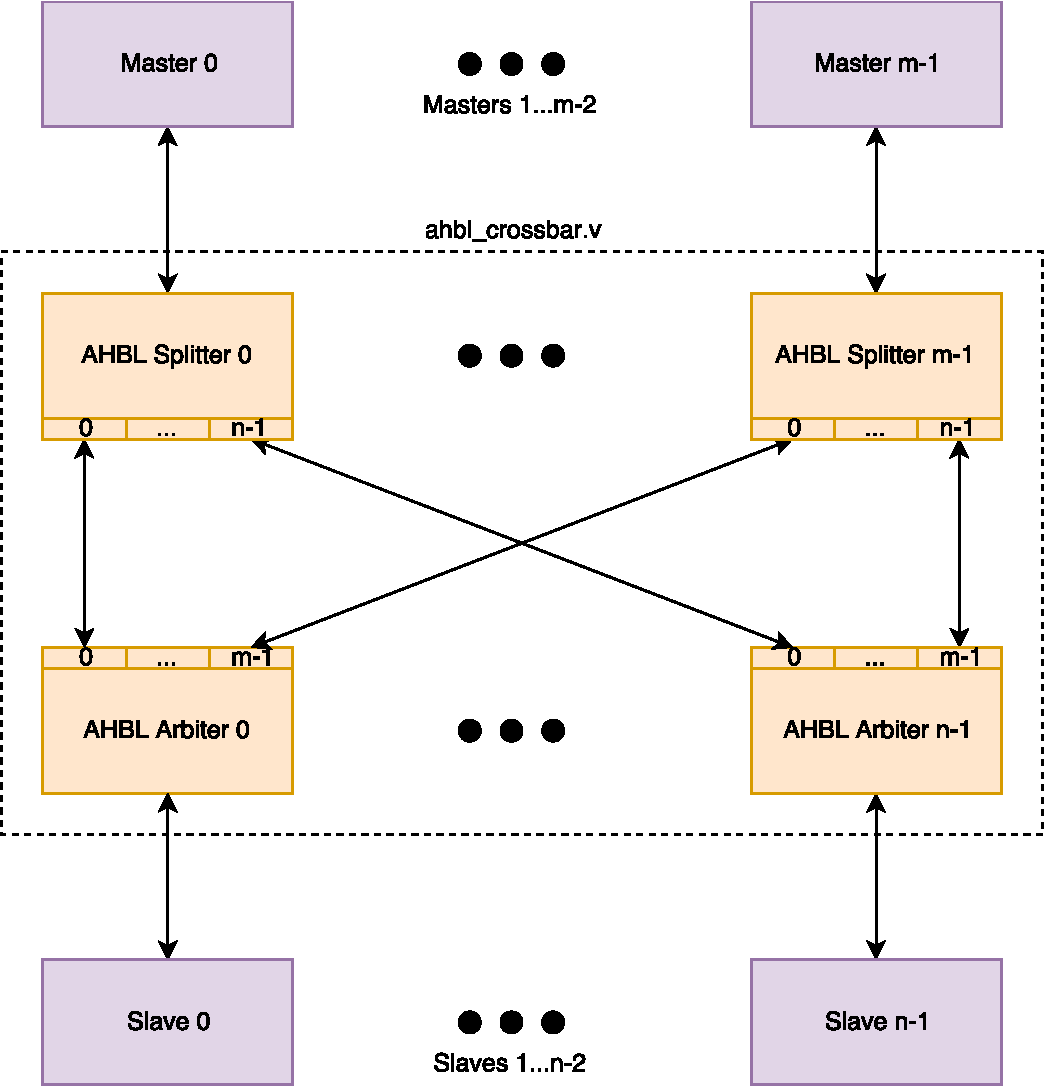
\includegraphics[width=0.6\textwidth]{diagrams/crossbar_structure.pdf}
\label{diagram:crossbar_structure}
\end{figure}

Each master is under the illusion that it is the only master in the system, but that slaves sometimes take longer to respond. During this waiting period, the slave may actually have fielded multiple transactions from higher-priority masters; this interaction handled by the slave's AHB-lite arbiter, and is transparent to the masters.

One of the crossbar's slave ports is attached to an AHBL-APB bridge. This bridge appears as a slave to the AHB portion of the bus fabric, and as a master to the APB portion. There are three main benefits to this scheme:

\begin{itemize}
	\item APB is fundamentally simpler
	\begin{itemize}
		\item This keeps peripheral gate count down
		\item The peripherals on the APB bus do not need the full AHB-lite bandwidth anyway
	\end{itemize}
	\item Fewer AHB-lite slaves
	\begin{itemize}
		\item There is a nonlinear area scaling associated with adding slaves to the AHB-lite fabric
		\item This would also add extra gate delays to a fairly critical data path
	\end{itemize}
	\item One APB master
	\begin{itemize}
		\item AHB-lite masters get arbitrated down to one inside the AHB-lite crossbar. APB slaves do not care who is addressing them.
		\item Different masters accessing different APB slaves will have to queue to use the bridge, even though they could theoretically proceed simultaneously
		\item However, area/complexity vs performance tradeoff is more than worth it for slow peripherals
		\item Multi-master APB is easy to implement, but never used in practice, due to the above tradeoff
	\end{itemize}
\end{itemize}

The splitter and arbiter modules in the AHB-lite crossbar can also be used on their own. Arbitrary multi-layer busfabric topologies should be possible with these two components.

Currently, the FPGABoy busfabric does not support AHB-lite bursts (TODO), and the masters do not use them.

\subsection{AHB-lite Primer}

For a full understanding of the bus standard used by FPGABoy, read through ARM's AMBA 3 AHB-lite spec. This document is mirrored in the \texttt{reference} folder in the GitHub repository, and gives a clear and comprehensive breakdown of AHB-lite. However, the following overview should provide sufficient understanding of the standard to read through the Verilog.

Masters assert requests onto the bus, and slaves assert responses. Each request can be either a read or a write, to some specified address. AHB-lite requires all transactions to be naturally aligned, i.e. the modulo of address and transfer size is zero. This is in tension with the RISC-V ISA which allows any transaction to have byte-alignment, so the load/store logic in the FPGABoy CPU must translate some load/store instructions into multiple AHB-lite transactions.

AHB-lite has separate data paths for read and write. This reflects a move away from tristate logic in ASIC bus designs, and a lack of tristate logic in FPGAs.

AHB-lite transactions take place in two phases, named the address phase and the data phase. During the address phase, the master asserts signals which control the nature of the transfer, such as the address, whether the transfer is a read or write, protection/permission information, the width of the data, and so on. During the data phase, data is asserted on either the read or write data bus (\texttt{hrdata} and \texttt{hwdata}), but never both.

The central conceit of AHB-lite is that these two phases are \textit{pipelined}. Whilst the master is asserting or accepting data for an earlier transaction (currently in data phase), it concurrently asserts address and control information for a later transaction (currently in address phase). As is generally the case with pipelining, the goal is to enable higher clock frequencies with undiminished work-per-clock.

\begin{figure}[H]
\centering
\caption{A simple AHB-lite example}
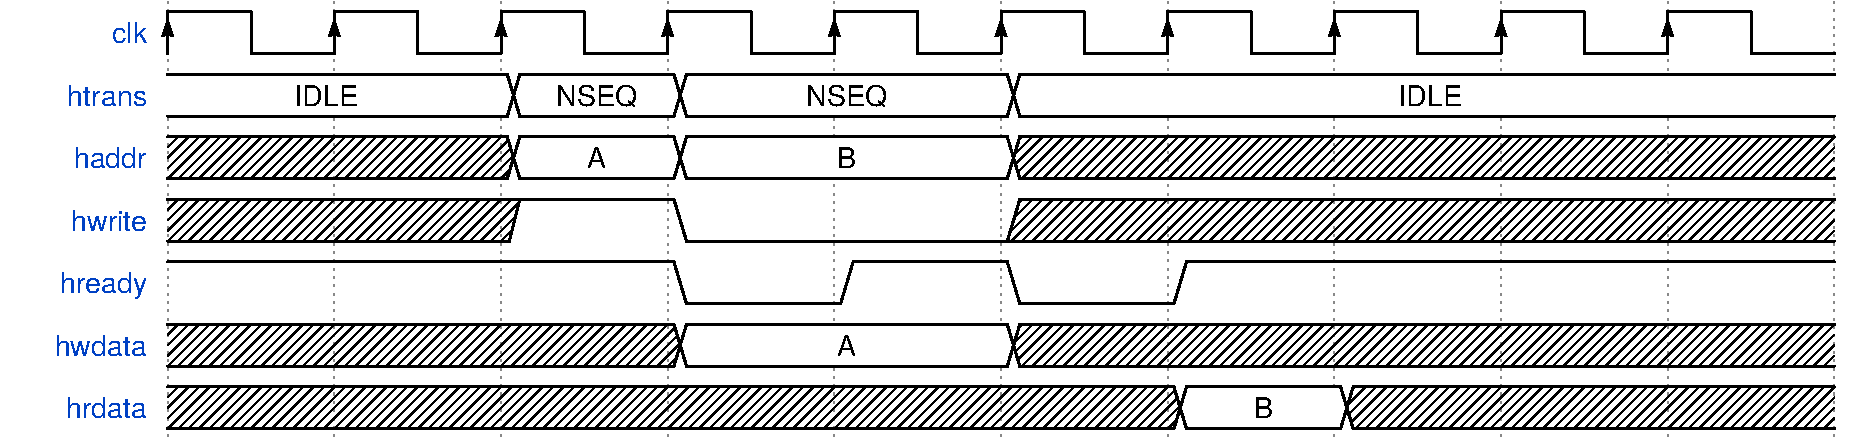
\includegraphics[width=0.9\textwidth]{waves/ahbl_basic.pdf}
\label{diagram:ahbl_basic}
\end{figure}

In figure \ref{diagram:ahbl_basic}, a master carries out two AHB-lite transactions: a write to address A, followed by a read from address B. Only a subset of AHB-lite signals are shown on the diagram.

\texttt{htrans}, \texttt{haddr}, and \texttt{hwrite} are address-phase signals, driven by the master; the other three are data-phase. \texttt{htrans} indicates the type of transfer the master next wishes to perform; allowed values are \texttt{IDLE}, \texttt{NSEQ} (non-sequential), \texttt{SEQ} and \texttt{BUSY}. The masters on FPGABoy only use \texttt{IDLE} and \texttt{NSEQ}. \texttt{hwrite} indicates the direction of the transaction, and \texttt{addr} the address (which is used for slave selection based on system memory map, and local address mapping inside of slaves).

\texttt{hready} signifies the end of the current data phase. As a result, the current address-phase transaction proceeds into data phase. Each slave has a signal called \texttt{hreadyout}, indicating that \textit{it} is ready, and the bus fabric selects the \texttt{hreadyout} of the current data-phase slave to be the global \texttt{hready}.

Initially, the bus is at rest. The master is asserting \texttt{IDLE} transactions. An \texttt{IDLE} data phase always completes in a single cycle. Therefore, the address phase for the first transaction -- write to address A -- also completes in a single cycle. When \texttt{htrans} is \texttt{IDLE}, the address-phase signals shown here are unimportant.

This slave needs two cycles to perform each data phase; perhaps it is an SRAM capable of running only at half the system clock speed. Therefore, \texttt{hready} is low for one cycle, and high for the second (last) cycle. The master drives \texttt{hwdata} for the duration of A's data phase, and waits for the slave to signal completion.

After 2 cycles, the data phase for address A completes. This is also the end of B's address phase. The data on \texttt{hrdata} is considered \textit{invalid} until the slave signals \texttt{hready}. During B's data phase, the master signals \texttt{IDLE}, as it has no further transactions to carry out after the read from B.

\subsection{Multi-Master Operation}

In a single-master busfabric, \texttt{hready} is a global signal, which causes the entire AHB-lite state machine (masters, slaves, fabric, the lot) to advance. Where multiple masters are concerned, \texttt{hready} is more subtle; in one respect, it is a per-master stall signal. At this point we need to be more specific about the relationship between \texttt{hreadyout} and \texttt{hready}.

Any AHB-lite slave port (of which there is one on the master side of the splitter, and $n$ on the master side of the arbiter) has a signal called \texttt{hreadyout}, which indicates the slave's readiness. Each of these ports also has a signal called \texttt{hready}, which indicates that the data phase is ending for the master who is connected to this slave (in either phase). \texttt{hready} is a function of \texttt{hreadyout}s and bus state.

In the single-layer crossbar on FPGABoy, each system AHB-lite slave is the slave of an arbiter, which is the slave of several splitters, each of which is the slave of a system master. As a general rule, the busfabric must filter system slaves' \texttt{hreadyout}s up to each system master, tie \texttt{hreadyout}s across to \texttt{hready}s at the very top of the busfabric, and then distribute these \texttt{hready} signals down to the correct system slaves.

\subsubsection{Arbiters Only}

The arbiters are the most complex busfabric component, and make up the bulk of the discussion, as we consider interactions between multiple masters and a single slave. However, there are additional complexities when we combine arbiters and splitters to build a crossbar, which are discussed in the next seciton.

In figure \ref{diagram:ahbl_mm_simult1}, two masters attempt to access a single slave simultaneously. Assume that master 0 always wins address-phase arbitration:

\begin{figure}[H]
\centering
\caption{Two masters access one slave.}
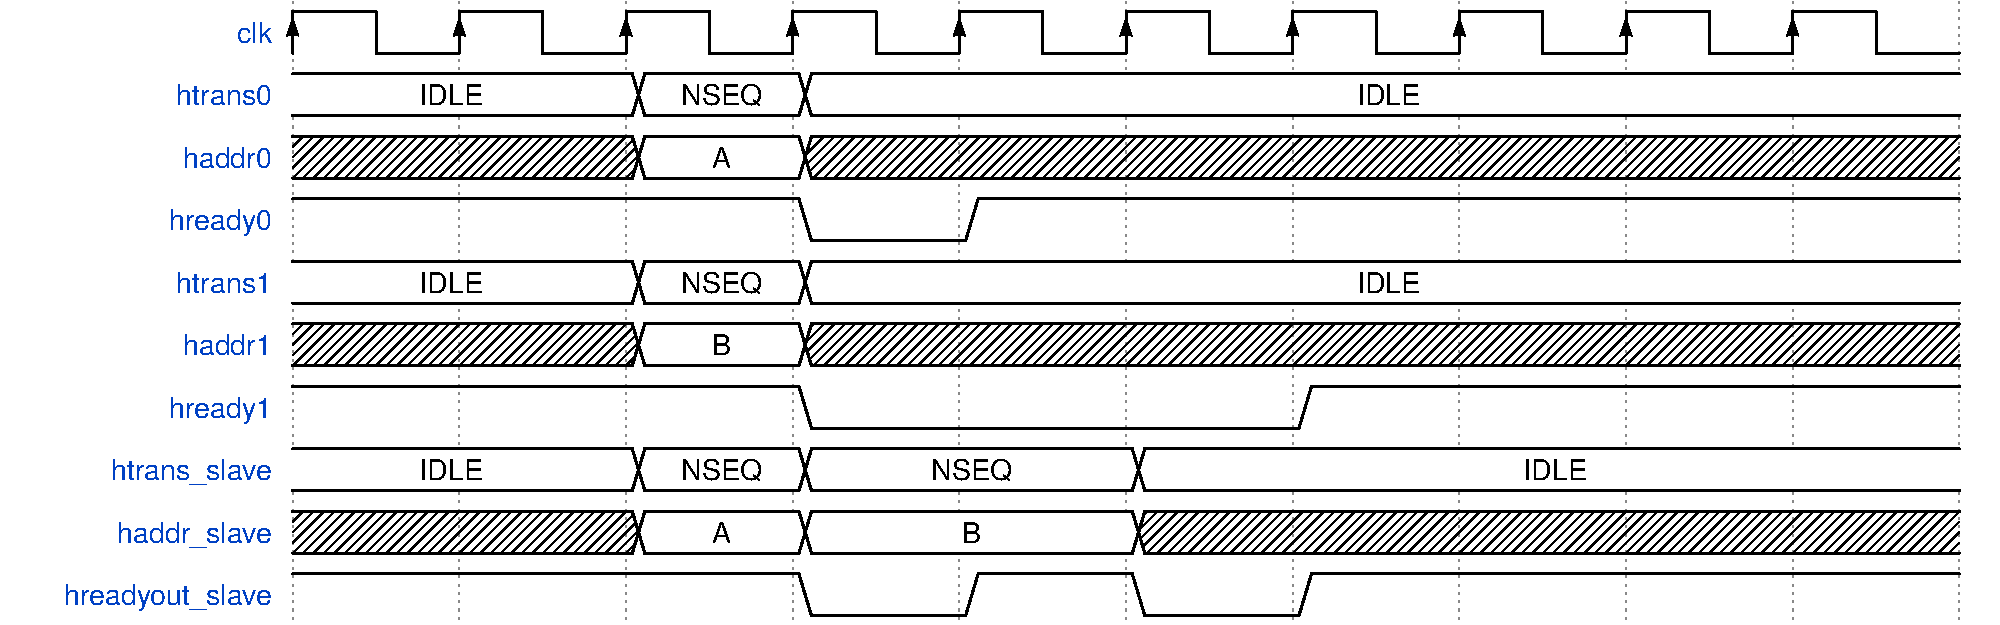
\includegraphics[width=0.9\textwidth]{waves/ahbl_mm_simult1.pdf}
\label{diagram:ahbl_mm_simult1}
\end{figure}

Again, we assume the slave requires 2 cycles to complete each data phase.

If we look at each master's trace, there is no indication at all that there is more than one master in the system: they present an address, and subsequently the transaction completes. Likewise, the slave neither knows nor cares that there are multiple masters: it simply carries out transactions according to the address-phase signals it sees. All of the smoke, mirrors and machinery are inside of the arbiter.

One odd feature of this trace is that, when the slave sees the address B, no master is asserting this address.

\begin{enumerate}
	\item Initially, both masters assert \texttt{IDLE}; \texttt{IDLE} data phases complete in one cycle
	\item \texttt{IDLE} data phases are concurrent with A, B address phases, so these \textit{also} complete immediately
	\item From the master 1's point of view, transaction B proceeds immediately to data phase.
	\item From both the master 0's and the slave's point of view, transaction A proceeds immediately to data phase
	\item Whilst the slave is in data phase for A, it is simultaneously in address phase for B
	\item When A data phase completes, master 0 is signaled, and B proceeds to data phase at the slave
	\item When B data phase completes, master 1 is signaled
\end{enumerate}

More concisely put, the first clock cycle of a given transaction's data phase may differ between the slave and master, but the \textit{last} cycle of that data phase is always the same clock cycle. The slave address phase will occur some time between the master address phase starting, and the slave data phase starting. These are strong enough guarantees for correct operation.

Based on this discussion, the AHB-lite arbiters need the facility to buffer one address-phase request, per master. A buffered request will be applied before any new requests from that master, but after any higher-priority requests. There is a nonzero hardware cost to this buffering, but there are clear engineering benefits to keeping this complexity confined to the arbiters, as they are the only component in the busfabric which is explicitly "multi master".

\begin{figure}[H]
\centering
\caption{Two masters access one slave, with low-priority back-to-back}
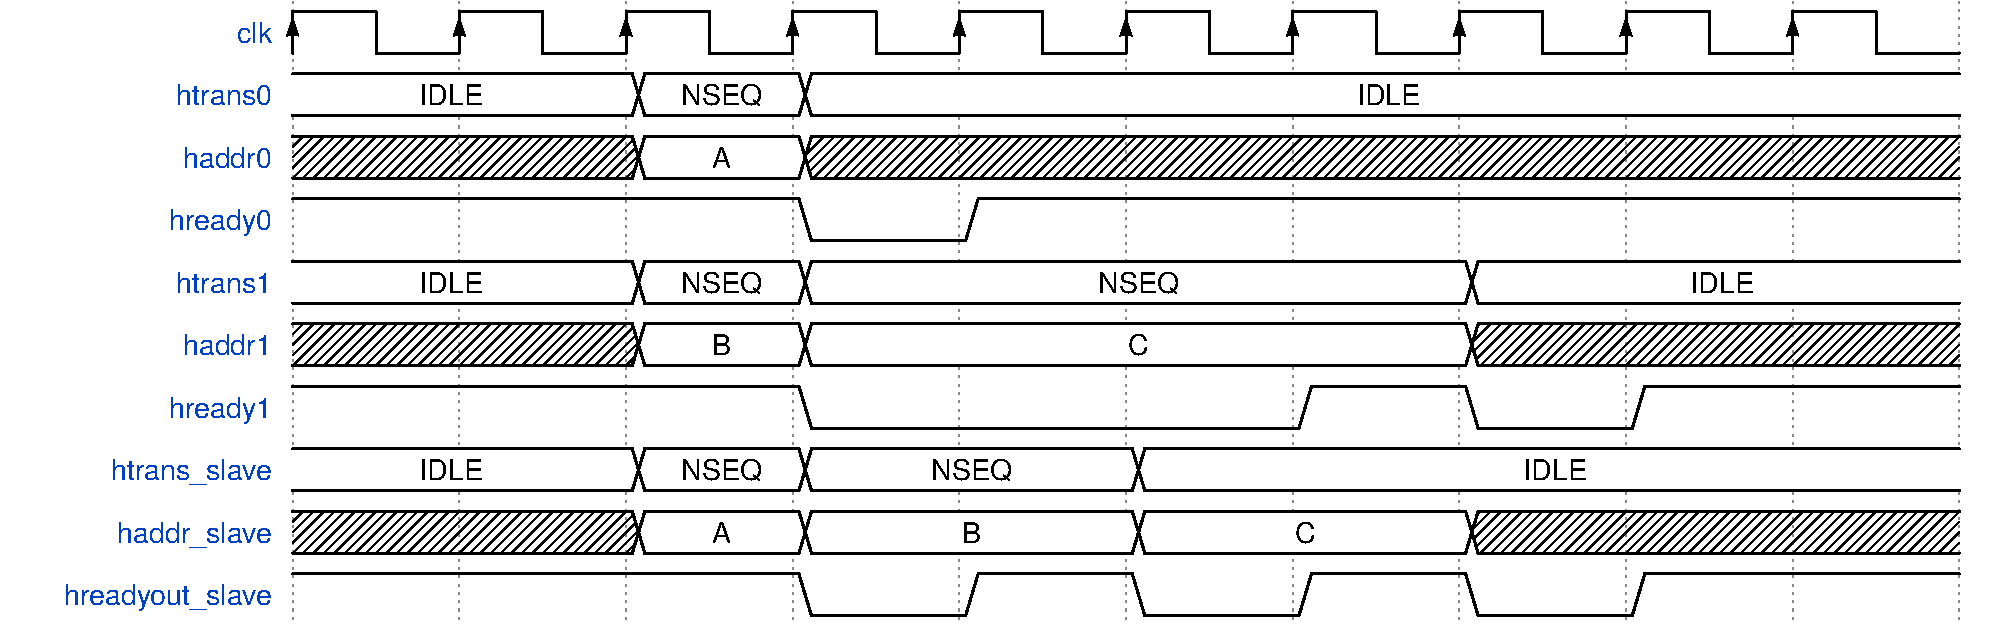
\includegraphics[width=0.9\textwidth]{waves/ahbl_mm_simult2.pdf}
\label{diagram:ahbl_mm_simult2}
\end{figure}

Figure \ref{diagram:ahbl_mm_simult2} shows the same sequence of events as figure \ref{diagram:ahbl_mm_simult1}, except master 1 now performs two back-to-back transactions. Once B's slave address phase completes, the arbiter's request buffer is cleared, and the C request passes transparently through the arbiter to the slave. Again, the only indication to master 1 of any master 0 activity is increased latency.

There is a different case which requires the arbiter's request buffer, shown in figure \ref{diagram:ahbl_mm_simult3}.

\begin{figure}[H]
\centering
\caption{Simultaneous request buffer writes}
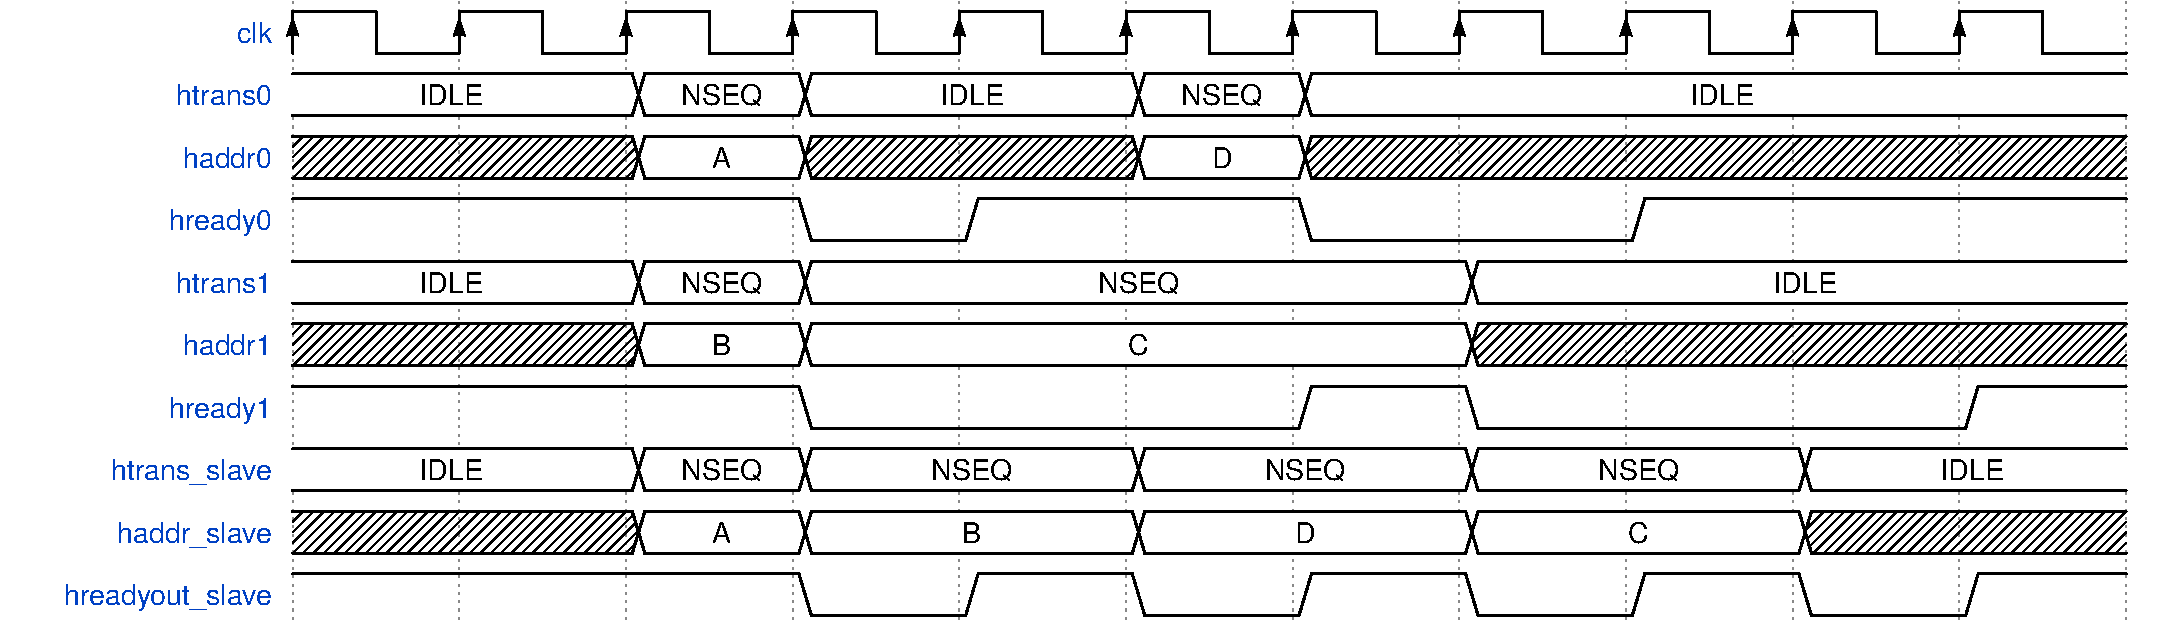
\includegraphics[width=0.9\textwidth]{waves/ahbl_mm_simult3.pdf}
\label{diagram:ahbl_mm_simult3}
\end{figure}

At the instant where D address phase is asserted, \texttt{hready0} is high, because master 0 previously asserted an \texttt{IDLE} transfer. However, the slave is not ready. In this case, the arbiter needs to buffer master 0's request, even though it is the highest-priority master. The buffered request is cleared once its slave address phase completes, as usual.

On the next cycle, B's data phase completes, and master 1 also considers this to be the end of the C address phase. The arbiter must write the C request into master 1's request buffer. Master 0's buffered request will continue to take priority over master 1's buffered request, until the first buffer is cleared.

There is one final case, for two masters accessing one slave, which is worth being aware of (figure \ref{diagram:ahbl_mm_latearrival}).

\begin{figure}[H]
\centering
\caption{High-priority late arrival}
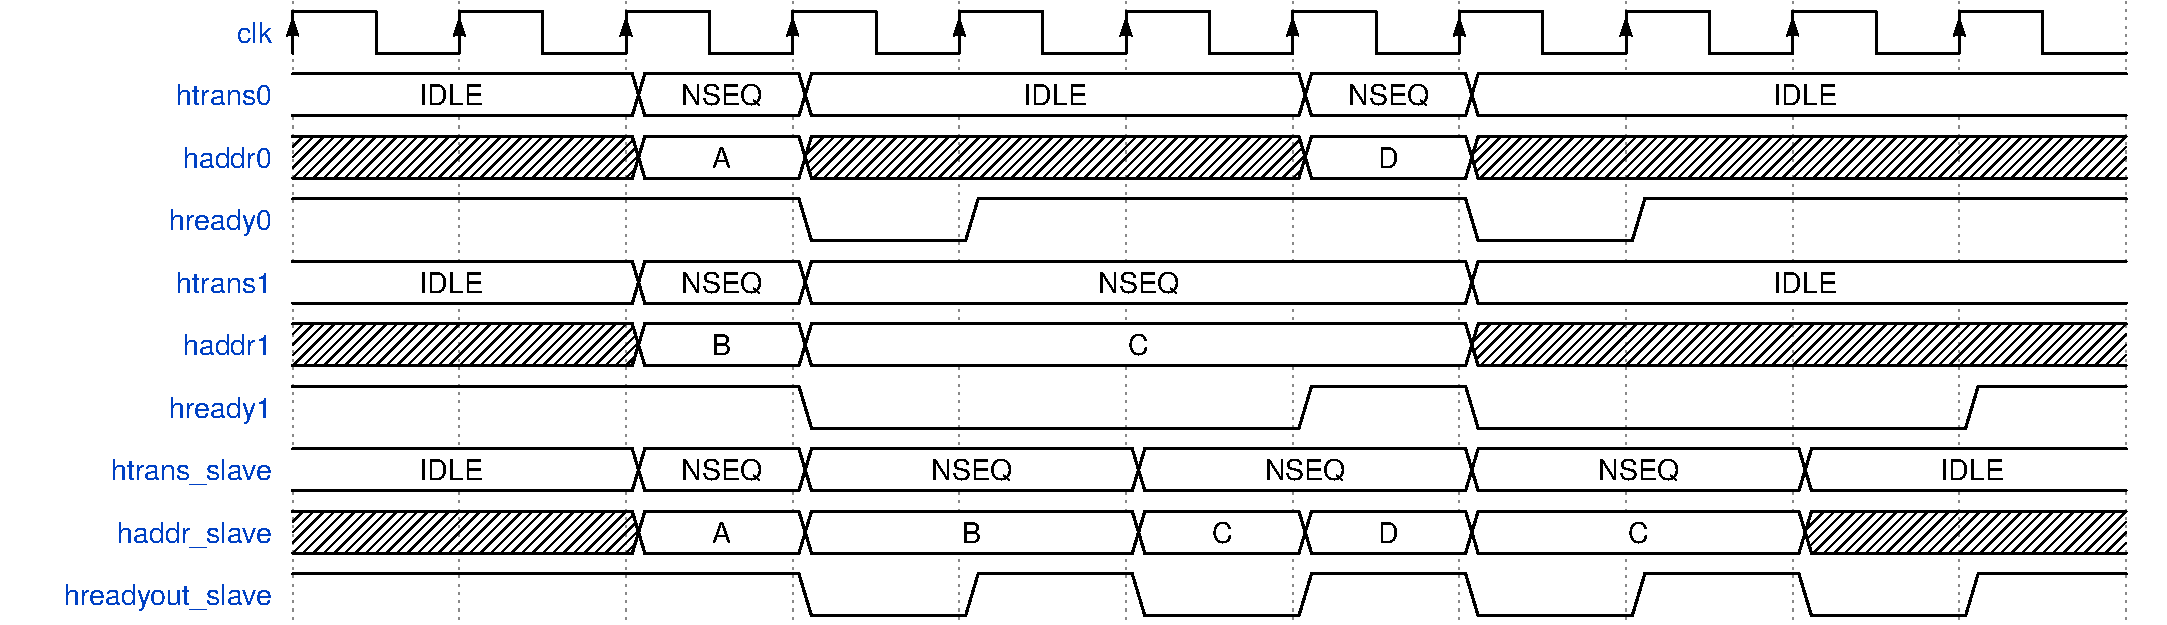
\includegraphics[width=0.9\textwidth]{waves/ahbl_mm_latearrival.pdf}
\label{diagram:ahbl_mm_latearrival}
\end{figure}

Whilst \texttt{hreadyout} is low, the C address briefly appears on the slave bus, before being replaced by the higher-priority D request. \textbf{This is a departure from the AHB-lite standard}, which stipulates the address must be constant during this time. This is deliberate, and easily amended. Slaves are generally insensitive to address-phase request during this time (as there is no performance benefit to latching APR before \texttt{hreadyout}, due to the way the bus operates), and this avoids a priority inversion, reducing average latency for higher-priority masters. If you find something that this breaks, write me an angry email! I would be interested to see such a slave.

The D request causes the low-priority C request to be buffered; the B data phase completes on this cycle, hence, from master 0's point of view, the C address phase does too.

\subsubsection{Full Crossbar}

The previous section discussed some cases where multiple masters access a single slave, and showed how the arbiter safely navigates them. There are yet more issues to consider when multiple masters and multiple slaves are involved, which must be handled without added latency cycles, and with minimal extra gate delay.

For example, a master may be engaged in address phase with one arbiter and data phase with another arbiter simultaneously, via a splitter, and these two arbiters will not necessarily signal \texttt{hreadyout} at the same time. Consequently, a master may have a positive \texttt{hready}, filtered from its data phase arbiter, when its address phase arbiter has a negative \texttt{hreadyout}, which requires action on the arbiter's part.

There is also the issue that being in data phase with an arbiter does not mean you are genuinely in data phase with the arbitrated slave; in fact, a very simple sequence of events (all masters \texttt{IDLE} $\to$ all masters \texttt{NSEQ}) will put all masters simultaneously in data phase with the same arbiter. The arbiter behaviour described in the previous section should allow us to abstract this away, provided we can deal with the first issue safely.

Hold onto your butts.

Splitters will filter their slaves' \texttt{hreadyout}s based on which is currently in data phase, and present it on their own slave port. Arbiters will present their slave's \texttt{hreadyout} on any master-facing ports which are in data phase with the arbiter, and will present $\texttt{hreadyout} = 1$ on any idle ports.

Splitters will fan their \texttt{hready} signal out to all of their slaves; a low \texttt{hready} directed at a slave you are not engaged with is harmless.


\section{Graphics Pipeline}

The graphics pipeline is still at the whiteboard stage, and its final form will depend on how many gates are left over when the rest of the system is finished. However, it will look something like the following (potentially without the affine transform blocks):

\begin{figure}[!htb]
\centering
\caption{Block-level diagram of graphics pipeline}
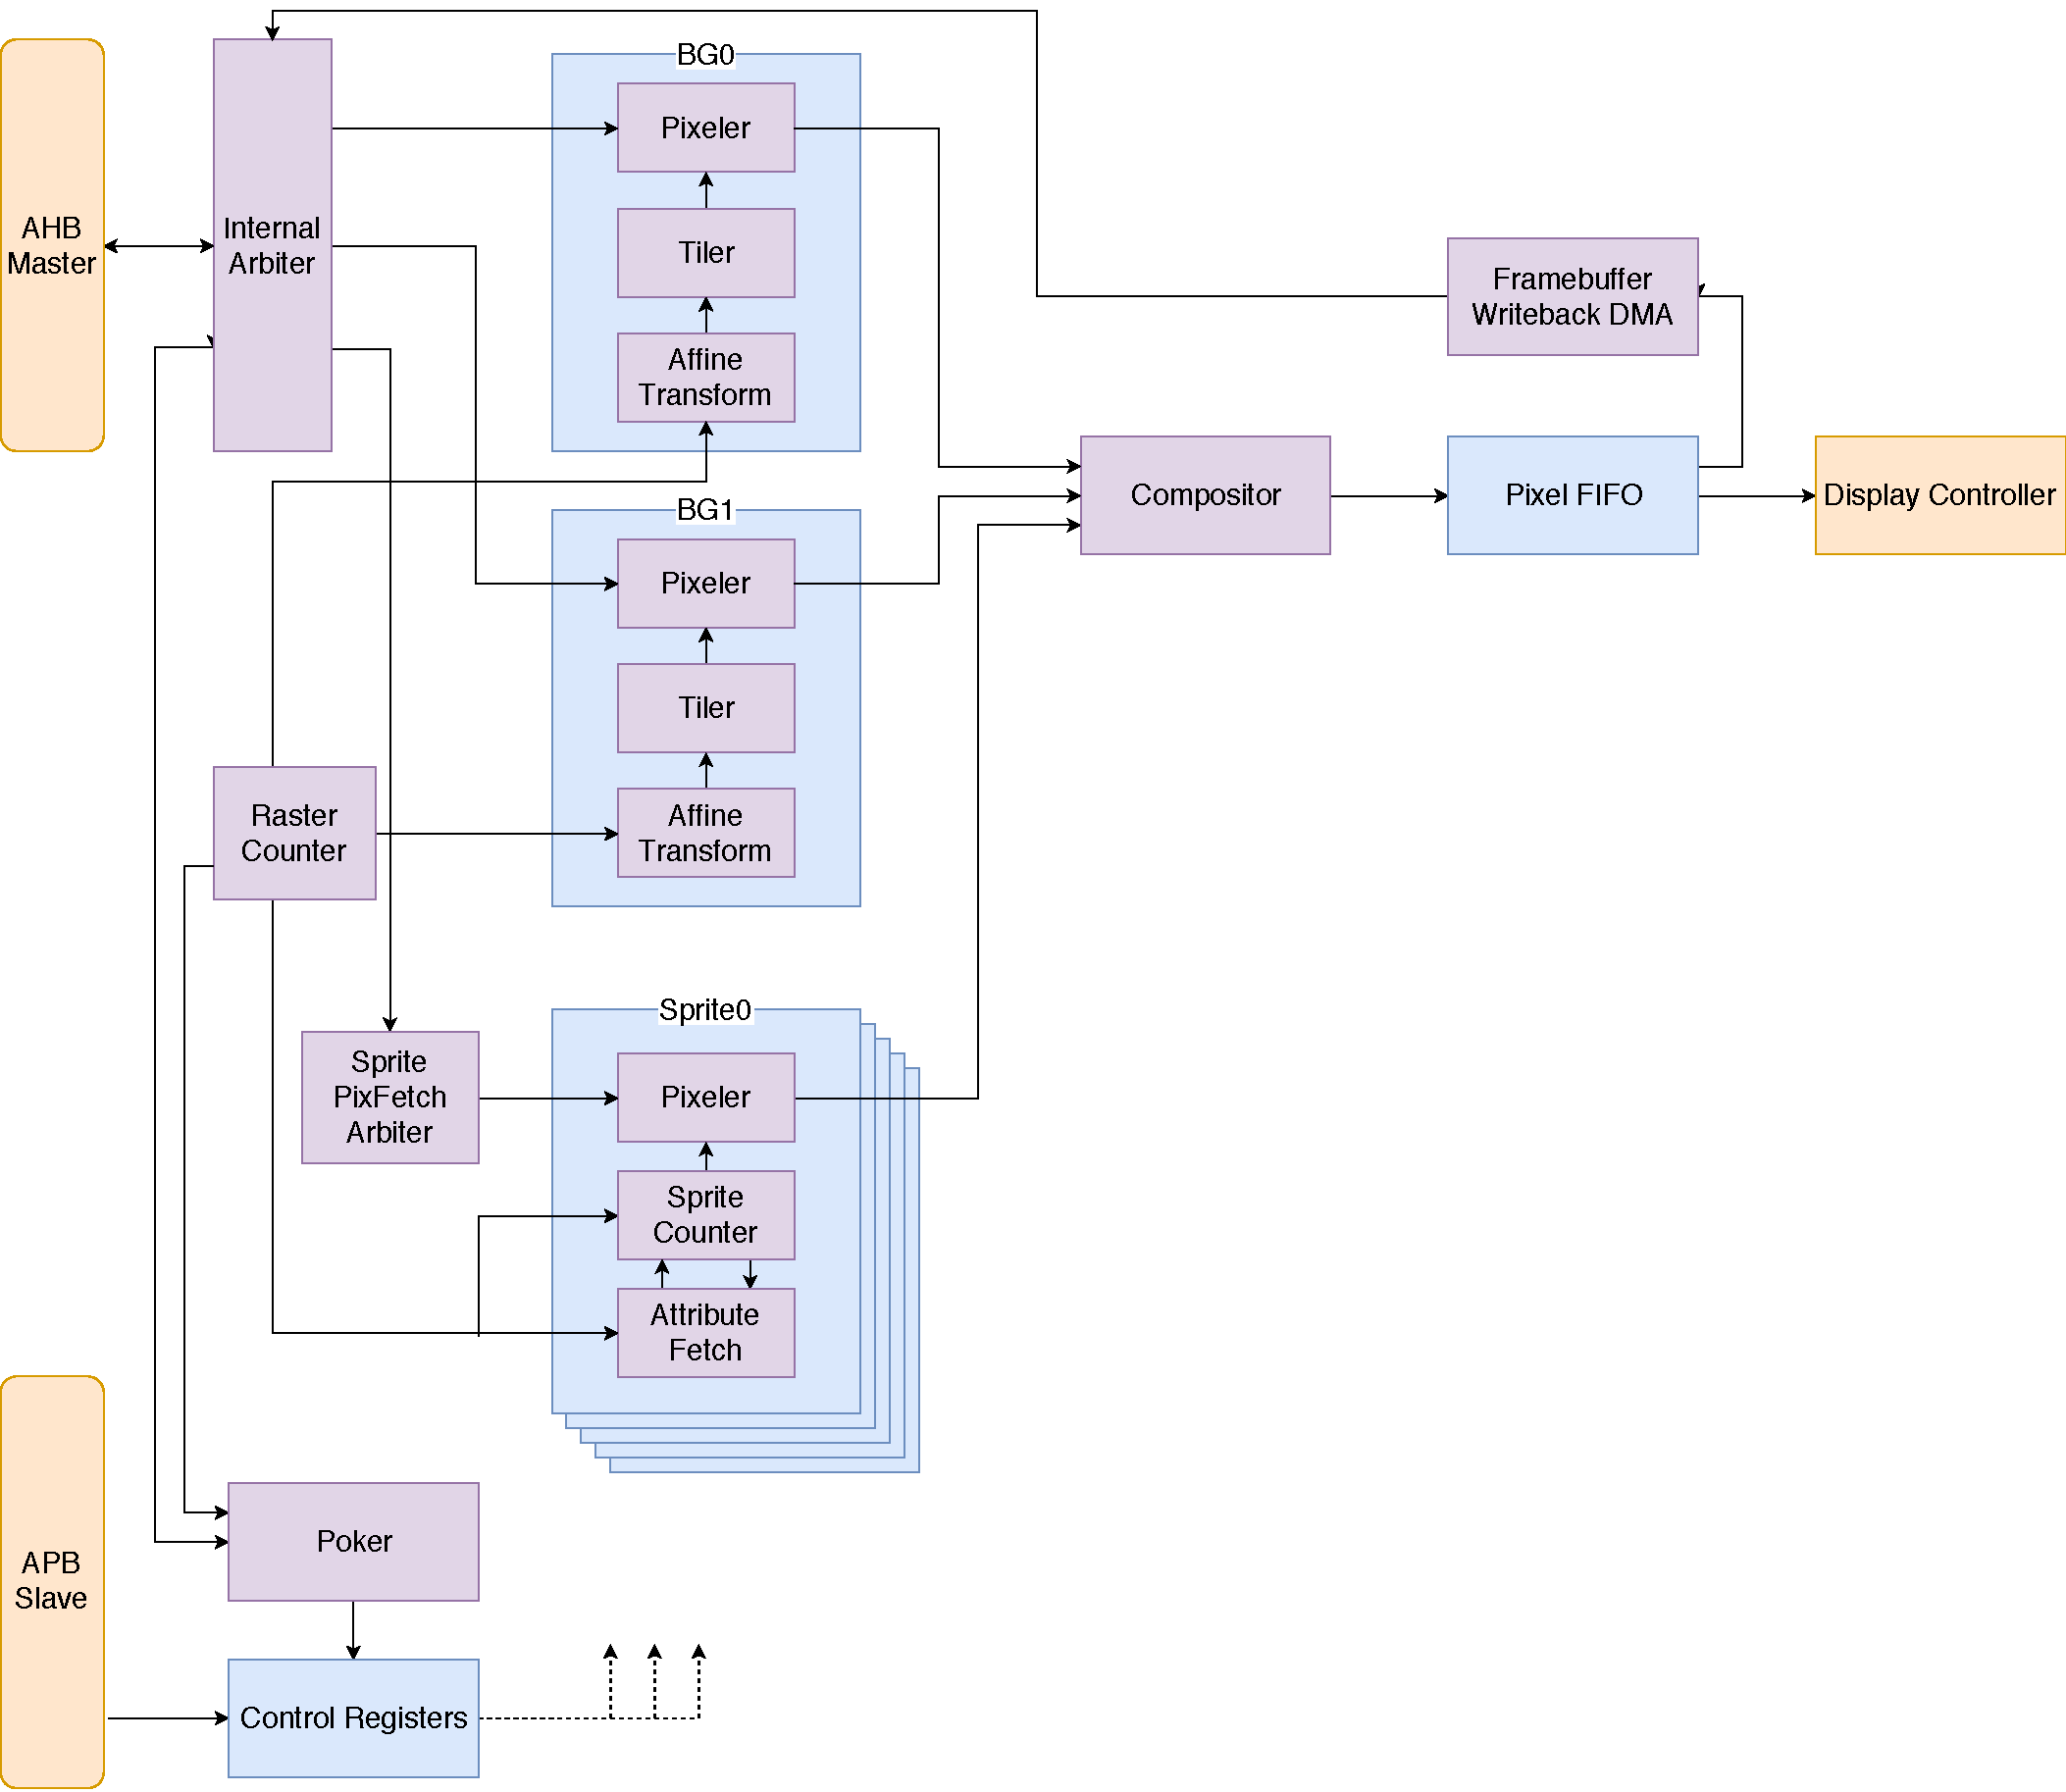
\includegraphics[width=0.9\textwidth]{diagrams/graphics.pdf}
\end{figure}

The poker is a simple raster-synchronised coprocessor which can poke control registers at precise points during a scanline, similar to the Copper on an Amiga. This would be particularly powerful in conjunction with background affine transform!

\end{document}